\documentclass{aci}

%%%%%%%%%%%%%%%%%%%%%%%%%%%%%%%%%%%%%%%%%%
\usepackage{txfonts}
\usepackage{booktabs}
\usepackage{longtable}
\usepackage{lipsum}
\usepackage{hyperref}
\usepackage{xcolor}
\hypersetup{colorlinks=true}
\usepackage{subcaption}
\usepackage{placeins}
\usepackage{tikz}
\usepackage{makecell}
\usetikzlibrary{automata,positioning,arrows}
\usepackage{caption}
\usepackage{changepage}

%%%%%%%%%%%%%%%%%%%%%%%%%%%%%%%%%%%%%%%%%%
\newcommand{\ep}{\varepsilon}
\newcommand{\eps}[1]{{#1}_{\varepsilon}}

\def\typeofarticle{Research Article} 
\def\currentvolume{3} 
\def\currentissue{1}
\def\currentyear{2022} 
\def\currentmonth{} 
\def\ppages{xx--xx} 
\def\DOI{xxxx} 
\def\Received{xx xx 2022} 
\def\Revised{xx xx 2022}
\def\Accepted{xx xx 2022} 
\def\Published{xx 2022}

\numberwithin{equation}{section}
\DeclareMathOperator*{\essinf}{ess\,inf}

\usepackage{array}
\newcolumntype{L}{>{\arraybackslash}m{8cm}}

\hyphenpenalty=10000
\usepackage{cite}
%%%%%%%%%%%%%%%%%%%%%%%%%%%%%%%%%%%%%%%%%%
\begin{document}

\title{Ant cuticle image classification using texture analysis: a comparative study}

\author{%
    Noah Gardner\affil{1},
    John Paul Hellenbrand\affil{2},
    Anthony Phan\affil{1},
    Evan Zhu\affil{1},
    Zhiling Long\affil{3},
    Min Wang\affil{2},
    Clint Penick\affil{2},
    and Chih-Cheng Hung\affil{1}\corrauth
}%

% \shortauthors is used in copyright information in the end of the paper
\shortauthors{the Author(s)}

\address{%
    \addr{\affilnum{1}}{Laboratory of Machine Vision and Security Research, %
        College of Computing and Software Engineering, Kennesaw State %
        University, Marietta GA, USA}%
    \addr{\affilnum{2}}{College of Science and Mathematics, Kennesaw State
        University, Kennesaw, GA, USA}%
    \addr{\affilnum{3}}{Department of Mathematics, Science, and Informatics,
        Mercer University, Atlanta, GA, USA}%
}
\corraddr{chung1@kennesaw.edu}

\editor{Pasi Fr\"{a}nti}

\begin{abstract}
    There is a large variety of ant species, and most species are diverse in
    terms of size, shape, behaviors, and especially cuticle textures. However,
    the significance of ant cuticle texture is not widely researched. Ant
    cuticle texture presumably provides some type of function, and therefore is
    useful to research for ecological applications and bioinspired designs. This
    research employs image texture analysis and deep machine learning to
    automatically group similar ant species based on morphological traits. We
    provide a comparative study of the performance of texture analysis methods
    on ant images. We evaluate the results of the classification methods with
    modern visualization techniques.
    \colorbox{green}{TODO: what is the result? experiments? data?}
\end{abstract}
\keywords{texture analysis; image processing; classification; machine learning;
    ant cuticle images; ecology}
\maketitle

\section{Introduction}
\colorbox{green}{TODO: refer to ant head images in a consistent way}

\colorbox{green}{TODO: refer to traditional/classical in a consistent way}

\colorbox{green}{TODO: change ideal and non-ideal to features identified by
    the biologist and to invalid features (background, etc.)}

Insects compose half of biodiversity and rank among the most dominant organisms
in terrestrial ecosystems \cite{sheikh_diverse_2017}. A key factor for the
ecological success of insects is their exoskeleton, also known as cuticle. The
cuticle protects insects from predation, provides structural support, prevents
desiccation, and serves as a canvas for advertising visual and chemical signals
\cite{gullan_insects_2009}. Research has heavily focused on the macrostructures
and internal chemical components that make the exoskeleton functional and more
recent work is being done to understand the functional aspects of external
cuticle micro sculpturing \cite{muthukrishnan_insect_2020,
    gunderson_insect_1989, watson_diversity_2017}.

Due to the extensive number of insect species, manual exploration of
insect-based information is difficult and often requires specialized expertise.
Therefore, automated entomology is gaining attraction by both biologists and
computer scientists and is expected to be a major contribution to the future of
insect-based research \cite{martineau_survey_2017}. One of the most commonly
used data types for insect analysis is image data. To develop an image-based
system for insect analysis, we can take advantage of existing work in general
image analysis methods.

We examine ants (\textit{Formicidae}) as they display an extreme diversity of
cuticle micro sculpturing across all subfamilies. Sculpturing ranges from
parallel longitudinal ridges to deep oval impressions to erratic protuberances.
The sculpturing has arisen convergently and independently throughout ant's
evolutionary history, which suggests some inherent function. Cuticle sculpturing
on ants may help increase strength and rigidness, resist abrasion, increase
internal and external surface area, resist microbial growth, and rear beneficial
anti-biotic producing bacteria \cite{johnson_effect_2011,
    bruckner_relationship_2017, currie_coevolved_2006}. These specific functions may
be associated with certain sculpturing types. In order to analyze those
functions, it is necessary to segment the image and group similar textures for
further analysis.

In image texture analysis methods, the general goal is to automatically
categorize an object into a set of objects with similar texture-based features.
Texture analysis has shown promising results in related fields, such as plant
identification \cite{boudra_plant_2018} \colorbox{green}{TODO: more references
    and examples}. With modern texture analysis methods, the categorization of ants
can be automated and the results can be used to study the influence of cuticle
texture on ant ecology.

Image texture analysis heavily depends on the spatial relationships among gray
levels of pixels \cite{hung_image_2019}. Hence, feature extraction method is
usually applied to the spatial relationship. The gray-level co-occurrence matrix
(GLCM) and local binary patterns (LBP) are two of methods which are based on the
spatial relationships to extracting features for this purpose
\cite{haralick_textural_1973, goos_gray_2000}. Traditional image texture
analysis can be divided into four categories: statistical, structural,
model-based, and transform-based methods \colorbox{green}{[references]}. In the
past decade, the deep learning network becomes the mainstream in image
classification and segmentation \cite{liu_bow_2019}. Compared with the
traditional method in which a kernel must be designed for extracting features,
the deep learning network can automatically extract the features by itself.

In this study, we used some of both approaches for our work on the ant images.

\colorbox{green}{TODO: Specifically, what approaches used? Why do we use image
    texture for ant images? What are the contributions?}


\colorbox{green}{TODO: briefly discuss results from the research}

\section{Related Work}

\colorbox{green}{TODO: introduce the section}

\subsection{Sculpturing Identification}
Taxonomists have developed extensive terminology describing ant cuticle
sculpturing as it is often a useful diagnostic trait to distinguish between
closely related ant species \cite{blaimer_taxonomy_2019,fisher_ants_2007}. The
definitive text on ant cuticle terminology — \textit{The Glossary of Surface
    Sculpturing} — contains over 100 terms to describe the cuticle sculpturing
patterns of ants \cite{harris_glossary_1979}. There is often substantial overlap
among terms, and closely related cuticle patterns are likely to be functionally
similar. For example, the definition for “imbricate” is, “partly overlapping and
appearing like shingles on a roof or scales on a fish,” which is difficult to
distinguish from the definition of tesselate, “made up of squares like a chess
board, either in sculpturing or in color.”

Cuticle sculpturing in ants has been explored thoroughly from a taxonomic
perspective; however, the function of nano and microstructures on insect
exoskeletons is a developing topic in entomology. Watson et al. review the
literature of cuticle nano and microstructure function and propose 21 possible
functions associated with these structures \cite{watson_diversity_2017}. Many of
these functions are related to structures not found in ants such as scales and
nanostructures. The review does include functions that may relate to ants such
as friction control, enhanced surface area, and increased hardness.  Watson et
al. also describe seven types of cuticle structures ranging from hairs and
scales to nano and micro structures \cite{watson_diversity_2017}. The cuticle
sculpturing of ants seems to fall within one type - complex microstructures.

The five broad functional groupings developed that describe the complex
microstructures found on ants were derived from reviewing the variation of
cuticle sculpturing across ants. These functional groupings were also reflected
in Harris as many terms could be grouped together based on similar definitions
and comparing the scanning electron microscope photographs provided in the
publication \cite{harris_glossary_1979}.

\colorbox{green}{TODO: how do we connect this section to image texture analysis?
    (why do we research this and why image texture) }

\subsection{Texture Analysis}
\colorbox{green}{TODO: A brief survey on image texture and cite Liu's
    IJCV2019 survey paper}

\subsection{Insect Classification}
In this section, we provide an overview of some insect classification methods.
Proposed insect classification methods seek to classify insects at different
hierarchical levels, such as species, genus, family, and order. Additionally,
some methods may classify insects at a combination of different hierarchical
levels. Insect classification methods can be applied to a variety of fields. In
agriculture, insect classification methods can be used to identify the presence
of pest insects in crops, which can inform crop managers in their choice of
pesticides and help prevent crop loss \cite{liu_pestnet_2019,
    kasinathan_machine_2021}.

Feng et al. \cite{feng_automated_2013} apply an automated system to classify
moth images based on semantic related visual attributes, which are defined as a
pattern on the moth wings. Feng et al. \cite{feng_automated_2013} use a custom
texture descriptor based on the combination of GLCM and \textit{scale-invariant
    feature transform} (SIFT) features \cite{gotlieb_texture_1990,
    lowe_distinctive_2004}. The method proposed by Feng et al.
\cite{feng_automated_2013} is used to classify 50 different moth species across
8 families \cite{feng_automated_2013}. The results from Feng et al.
\cite{feng_automated_2013} suggest that traditional feature extraction
techniques for the semantic visual attributes of the moth wings are sufficient
for training a classifier to classify an image between 10 randomly selected moth
species.

Urteaga et al. \cite{urteaga_scorpions_2016} use machine learning methods in
order to classify images between two different scorpion species:
\textit{Centruroides limpidus} and \textit{Centruroides noxius}. After applying
background distinction based on dynamic color threshold, Urteaga et al.
\cite{urteaga_scorpions_2016} apply feature extraction to extract features from
the separated scorpion image such as aspect ratio, rectangularity, and
compactness. Urteaga et al. \cite{urteaga_scorpions_2016} apply three different
classification models to classify the image as one of the species: Artificial
Neural Network, Regression Tree, and Random Forest classifiers
\cite{urteaga_scorpions_2016}. The results from Urteaga et al.
\cite{urteaga_scorpions_2016} show that after background removal,
characteristics from the entire body of the scorpion can be used to create a
binary classifier that can classify the image as one of the two species.

Lim et al. \cite{lim_performance_2017} apply a CNN-based algorithm for insect
classification. Lim et al. \cite{lim_performance_2017} classify a subset of
insect species and families based on the classes available in the ImageNet
dataset. ImageNet is a widely used dataset of images labeled by experts with
millions of images and thousands of categories \cite{deng_imagenet_2009}. In the
ImageNet dataset, there are some categories that specify the class of the insect
on a species level, \textit{e.g.} \textit{monarch butterfly} and \textit{ringlet
    butterfly} as well as some categories that specify the class of the insect on a
family level, \textit{e.g.} \textit{ant}, \textit{fly}, and \textit{bee}
\cite{imagenet_labels}. Lim et al. \cite{lim_performance_2017} use a modified
AlexNet architecture and experiment with different numbers of kernels and their
effect the performance of the model. Glick et al. \cite{glick_insect_2016}
employ a similar approach by classifying 277 insect classes from ImageNet using
a hierarchical convolutional neural network. The results from Lim et al.
\cite{lim_performance_2017} and Glick et al. \cite{glick_insect_2016} suggest
that a CNN is capable of differentiating between different hierarchical classes
of insects.

\section{Methodology}

\colorbox{green}{TODO: do not jump into subsection directly without any context}

\subsection{Dataset preparation} % preparation generation

\begin{figure}[h]
    \centering
    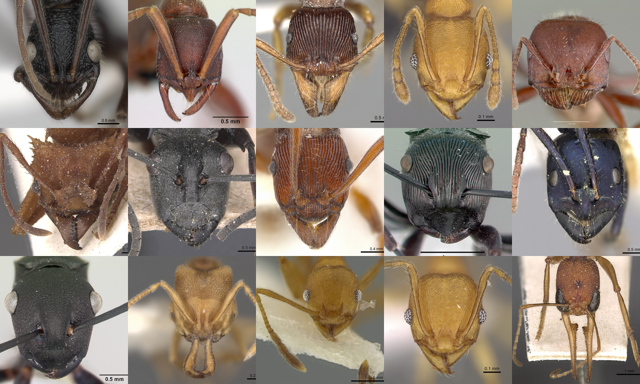
\includegraphics[width=0.7\textwidth]{thesis_assets/images/rough_collage.png}
    \caption{Examples of rough cuticle texture ant images in the dataset after
        center cropping, from AntWeb \cite{perrichot_antweb_2012}.}
    \label{fig:rough-cuticle-texture}
\end{figure}

In this section, we describe the creation of the custom dataset used in this
research. In our dataset, we use ant head images from AntWeb
\cite{perrichot_antweb_2012} and define two categories for them based on the
appearance of the cuticle texture: \textit{rough} and \textit{smooth}. Some
randomly selected images from each category are shown in Figures
\ref{fig:rough-cuticle-texture} and \ref{fig:smooth-cuticle-texture}.

\begin{figure}
    \centering
    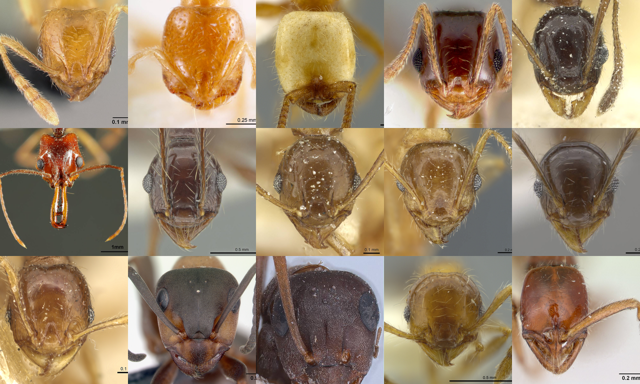
\includegraphics[width=0.7\textwidth]{thesis_assets/images/smooth_collage.png}
    \caption{Examples of smooth cuticle texture ant images in the dataset after
        center cropping, from AntWeb \cite{perrichot_antweb_2012}.}
    \label{fig:smooth-cuticle-texture}
\end{figure}

% \subsubsection{Sculpture identification protocol}

To begin, a master spreadsheet was created with the 2,499 different ant species
to be identified for the primary dataset. The team was trained to identify
cuticle sculpturing through a process which consisted of one 45-minute
introductory lesson explaining the project and texture categories. Then, the
team was given a training set of photos to identify from the genus
\textit{Polyrhachis}. The sculpture identification protocol describes the two
primary categories: \textit{rough} and \textit{smooth}.

Initially, the sculpture identification protocol had 8 subcategories of cuticle
texture, including dimpled, ridged, and differing levels of smooth texture. For
simplicity, we work only with the two main categories. The training set
identifications were reviewed together as a group by the assistants. Once
training was complete, assistants were assigned the same genera of ants to
identify independently each week. A weekly meeting was held to discuss
identifications and assign new ones. These identifications were collected in the
master spreadsheet and the identifications were assigned to individual ant
species on a majority basis.

% \subsubsection{Data collection}

To collect the images, the assistants followed the taxonomy information
available in the master spreadsheet to the appropriate AntWeb page
\cite{perrichot_antweb_2012}. In many cases, there are multiple ant head images
of the same species, and occasionally there are multiple image resolution
available from a single image. To simplify the data collection process, the
assistants were instructed to download the first ant head image of the species
being identified in the highest resolution possible. Each image was named with
an identifier that corresponds with the row number in the master spreadsheet.
The same ant head images that were downloaded in the data collection phase were
the same ones used in the sculpture identification protocol. Ant species which
did not have any images of the head were excluded from the dataset.
Additionally, ant species which only had a head image of a queen ant were
excluded from the dataset.

Ant specimen images taken from AntWeb \cite{perrichot_antweb_2012} are created
by different photographers and therefore have different attributes, such as
environment, resolution, and lighting. In the ant head images, the ant head is
in the center of the image and the body is pointing away from the camera. The
focus of the ant head image is centered on the head, with the background and
image artifacts from the ant body typically blurred. In most ant head images,
there is a bar which indicates the scale of the image due to the variety in the
sizes of different ant species. In a few ant head images, there exists some text
denoting the specimen identifier and other information. In terms of texture,
some ant specimens are very old, so their head images have other abnormalities
such as cracks in the cuticle and the presence of dust.

% \subsubsection{Data preprocessing}

Due to the variety of the ant head image attributes, we apply simple
preprocessing before the images are used in our model. We want the images to
have a uniform size for simplicity in our classification process. Since the ant
head images are typically centered in the image, we apply a center crop to each
image to create a square image of the same size. Once the image is square, we
resize each image to a fixed size of 256x256 pixels. We leave other
discrepancies in the images untouched.

Our custom dataset of ant head images contains 2,499 images. 1072 samples of
rough textured ant cuticle textures comprise 43\% of the dataset. The remaining
1427 samples of smooth textured ant cuticle textures comprise 57\% of the
dataset. To handle the imbalance of the dataset, we apply undersampling for each
class for the training dataset. By using random stratified sampling, we
construct a training set with 800 images per class. The remaining images are
randomly split between test and validation, which turns out to roughly a
60\%/20\%/20\% train, test, and validation data split. With 272 rough samples
and 627 smooth samples left over after the stratified split, the test dataset
has roughly 136 rough samples and 313 smooth samples. Since these leftover
samples are split with code by 50\% there will be some rounding variance and
therefore the test dataset built at run-time will not always have exactly the
same number of samples.

\subsection{Classical texture analysis methods}

\colorbox{green}{TODO: kviews, gabor, etc. will go here}

\subsection{Deep learning models used for the experiments}

Our first model is \textit{visual geometry group} (VGG), a convolutional neural
network that takes advantage of very small convolutional filters in a deep
network architecture \cite{simonyan_very_2015}. We compare four architectures of
VGG: VGG11, VGG13, VGG16, and VGG19. The primary difference between the
architectures is the number of layers in each model. Our second model is
\textit{residual network} (ResNet), a deep network architecture that includes
shortcut connections between layers (residual connections) \cite{he_deep_2015}.
We compare three architectures of ResNet: ResNet18, ResNet50, and ResNet101.
Again, the primary difference between the architectures is the number of layers
in each model.

For our ResNet models, we have two versions: randomized and pretrained. The
randomized version is the same architecture, but the weights are randomly
initialized. The pretrained version has weights from training on the CIFAR
dataset, an image dataset with 1000 classes. In this case, we are fine-tuning
the pretrained model. For VGG, we are only using the randomized version. The
base VGG architecture also has an output layer of size 1000. Since we are
working with a binary classification problem, we modify the architecture for all
models to have an output layer of size 2. Each model is trained over 100 epochs,
using stochastic gradient descent with momentum. The batch size is set to 16
images. We apply a learning rate of 0.001 and momentum parameter of 0.9.

\colorbox{green}{\parbox{\dimexpr\textwidth-2\fboxsep}{TODO: I suggest that
        at least one deep learning based texture classification algorithm be applied
        to the dataset for the comparative study. When this is the case, one more
        subsection should be included here to describe that/those algorithm(s).}}

\subsection{Evaluation}

We evaluate the performance of the models according to standard evaluation
methods. Since we are working with a binary classification problem, we use a
standard confusion matrix to evaluate the accuracy, precision, and F1 score.
\colorbox{green}{(TODO: AUC and ROC can also be used as additional evaluation
    methods.)} We also apply Grad-CAM with manual inspection to visualize the
activation weights for classified images to visualize which features lead to the
classification result. Finally, we apply t-SNE to visualize the separation
learned for the model to further analyze the classifications made by the model.

\section{Results}
\subsection{Environment}

Experiments are run on an Ubuntu 18.04 LTS Lambda Labs GPU server. The server
contains 8 NVIDIA GeForce RTX 2080 Ti graphics cards with 12GB of memory each.
The server uses an Intel Xeon Silver 4116 with 48 total threads and maximum
frequency of 3.000 GHz, and has 256GB of RAM.

% vgg results
\subsection{VGG Models}

To begin, we share the results on the VGG model architectures on our custom
dataset. The classification results are summarized in a confusion matrix for
each model. Then, the statistics for each VGG architecture are shared in Table
\ref{tab:vgg_results}. The results are collected on 8 runs of training and
averaged. The results are rounded to 2 decimal places where appropriate.

% \begin{table}[h]
%     \centering
%     \caption{VGG11 confusion matrix on ant head image dataset.}
%     \begin{tabular}{r|ll}
%                          & True Rough & True Smooth \\
%         \hline
%         Predicted Rough  & 101.75     & 53          \\
%         Predicted Smooth & 37.375     & 257.875     \\
%     \end{tabular}
%     \label{tab:vgg11_confusion_matrix}
% \end{table}

% \begin{table}[h]
%     \centering
%     \caption{VGG13 confusion matrix on ant head image dataset.}
%     \begin{tabular}{r|ll}
%                          & True Rough & True Smooth \\
%         \hline
%         Predicted Rough  & 95.25      & 39.375      \\
%         Predicted Smooth & 43.25      & 272.25      \\
%     \end{tabular}
%     \label{tab:vgg13_confusion_matrix}
% \end{table}

% \begin{table}[h]
%     \centering
%     \caption{VGG16 confusion matrix on ant head image dataset.}
%     \begin{tabular}{r|ll}
%                          & True Rough & True Smooth \\
%         \hline
%         Predicted Rough  & 87.5       & 42.625      \\
%         Predicted Smooth & 47.375     & 272.5       \\
%     \end{tabular}
%     \label{tab:vgg16_confusion_matrix}
% \end{table}

% \begin{table}[h]
%     \centering
%     \caption{VGG19 confusion matrix on ant head image dataset.}
%     \begin{tabular}{r|ll}
%                          & True Rough & True Smooth \\
%         \hline
%         Predicted Rough  & 91.25      & 42.125      \\
%         Predicted Smooth & 43.25      & 273.375     \\
%     \end{tabular}
%     \label{tab:vgg19_confusion_matrix}
% \end{table}

\begin{table}[h]
    \centering
    \caption{Average results for VGG architectures on ant head image dataset.}
    \begin{tabular}{r|llll}
              & Recall & Precision & F1 Score & Accuracy \\
        \hline
        VGG11 & 0.83   & 0.88      & 0.85     & 0.80     \\
        VGG13 & 0.87   & 0.87      & 0.87     & 0.82     \\
        VGG16 & 0.86   & 0.86      & 0.86     & 0.80     \\
        VGG19 & 0.87   & 0.87      & 0.87     & 0.81     \\
    \end{tabular}
    \label{tab:vgg_results}
\end{table}

% \begin{figure}[h]
%     \centering
%     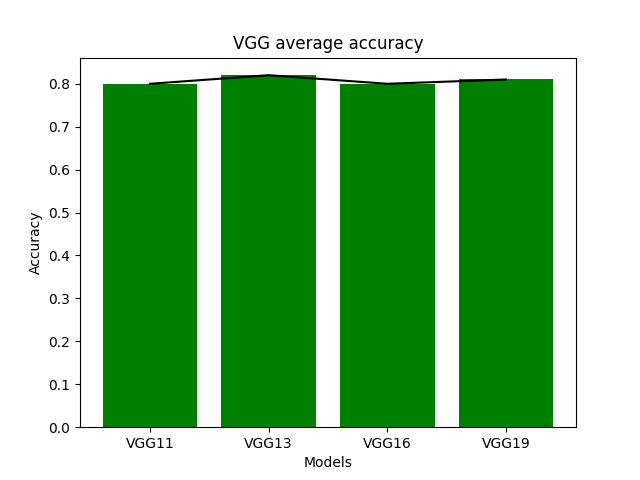
\includegraphics[width=0.6\textwidth]{thesis_assets/plots/vgg_average.png}
%     \caption{Average accuracy for VGG architectures on ant head image dataset.}
%     \label{fig:vgg_results}
% \end{figure}

\subsection{ResNet Models}

Next, we share the results on the ResNet model architectures on our custom
dataset with random weight initialization. The classification results are
summarized in a confusion matrix for each model. Then, the statistics for each
ResNet architecture are shared in Table \ref{tab:resnet_results}. The results
are collected on 8 runs of training and averaged. The results are rounded
to 2 decimal places where appropriate.

% \begin{table}[h]
%     \centering
%     \caption{ResNet18 confusion matrix on ant head image dataset.}
%     \begin{tabular}{r|ll}
%                          & True Rough & True Smooth \\
%         \hline
%         Predicted Rough  & 98.75      & 48.75       \\
%         Predicted Smooth & 39.25      & 262         \\
%     \end{tabular}
%     \label{tab:resnet18_confusion_matrix}
% \end{table}

% \begin{table}[h]
%     \centering
%     \caption{ResNet50 confusion matrix on ant head image dataset.}
%     \begin{tabular}{r|ll}
%                          & True Rough & True Smooth \\
%         \hline
%         Predicted Rough  & 81.375     & 43.625      \\
%         Predicted Smooth & 55.875     & 269.125     \\
%     \end{tabular}
%     \label{tab:resnet50_confusion_matrix}
% \end{table}

% \begin{table}[h]
%     \centering
%     \caption{ResNet101 confusion matrix on ant head image dataset.}
%     \begin{tabular}{r|ll}
%                          & True Rough & True Smooth \\
%         \hline
%         Predicted Rough  & 85.75      & 53.875      \\
%         Predicted Smooth & 50.125     & 260.25      \\
%     \end{tabular}
%     \label{tab:resnet101_confusion_matrix}
% \end{table}

\begin{table}[h]
    \centering
    \caption{Average results for ResNet architectures on ant head image dataset.}
    \begin{tabular}{r|llll}
                  & Recall & Precision & F1 Score & Accuracy \\
        \hline
        ResNet18  & 0.84   & 0.87      & 0.85     & 0.80     \\
        ResNet50  & 0.86   & 0.83      & 0.84     & 0.77     \\
        ResNet101 & 0.83   & 0.84      & 0.83     & 0.76     \\
    \end{tabular}
    \label{tab:resnet_results}
\end{table}

% \begin{figure}[h]
%     \centering
%     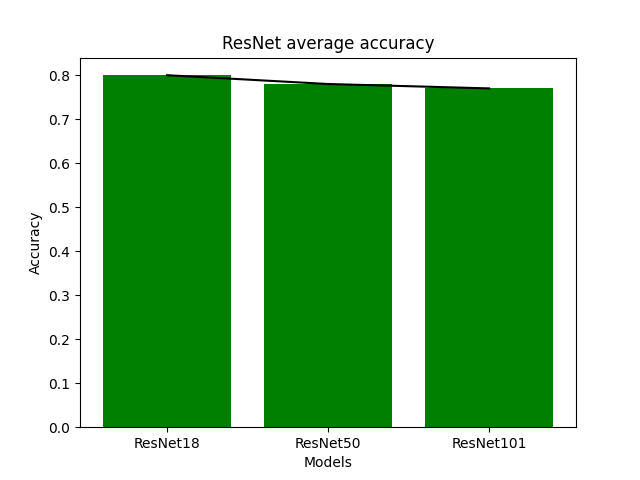
\includegraphics[width=0.6\textwidth]{thesis_assets/plots/resnet_average.png}
%     \caption{Average accuracy for ResNet architectures on ant head image dataset.}
%     \label{fig:resnet_results}
% \end{figure}

\clearpage
\subsection{Fine-tuned ResNet Models}

Next, we share the results on the fine-tuned ResNet model architectures on our
custom dataset with pretrained weights. The classification results are
summarized in a confusion matrix for each model. Then, the statistics for each
ResNet architecture are shared in Table \ref{tab:fresnet_results}. The results
are collected on 8 runs of training and averaged. The results are rounded
to 2 decimal places where appropriate.

% \begin{table}[h]
%     \centering
%     \caption{Fine-tuned ResNet18 confusion matrix on ant head image dataset.}
%     \begin{tabular}{r|ll}
%                          & True Rough & True Smooth \\
%         \hline
%         Predicted Rough  & 117.375    & 35.125      \\
%         Predicted Smooth & 17.875     & 279.625     \\
%     \end{tabular}
%     \label{tab:fresnet18_confusion_matrix}
% \end{table}

% \begin{table}[h]
%     \centering
%     \caption{Fine-tuned ResNet50 confusion matrix on ant head image dataset.}
%     \begin{tabular}{r|ll}
%                          & True Rough & True Smooth \\
%         \hline
%         Predicted Rough  & 114.5      & 33.25       \\
%         Predicted Smooth & 24.125     & 278.125     \\
%     \end{tabular}
%     \label{tab:fresnet50_confusion_matrix}
% \end{table}

% \begin{table}[h]
%     \centering
%     \caption{Fine-tuned ResNet101 confusion matrix on ant head image dataset.}
%     \begin{tabular}{r|ll}
%                          & True Rough & True Smooth \\
%         \hline
%         Predicted Rough  & 117.25     & 33.25       \\
%         Predicted Smooth & 18.375     & 281.125     \\
%     \end{tabular}
%     \label{tab:fresnet101_confusion_matrix}
% \end{table}

\begin{table}[h]
    \centering
    \caption{Average results for Fine-tuned ResNet architectures on ant head image dataset.}
    \begin{tabular}{r|llll}
                  & Recall & Precision & F1 Score & Accuracy \\
        \hline
        ResNet18  & 0.89   & 0.94      & 0.91     & 0.88     \\
        ResNet50  & 0.89   & 0.92      & 0.91     & 0.87     \\
        ResNet101 & 0.89   & 0.94      & 0.92     & 0.88     \\
    \end{tabular}
    \label{tab:fresnet_results}
\end{table}

% \begin{figure}[h]
%     \centering
%     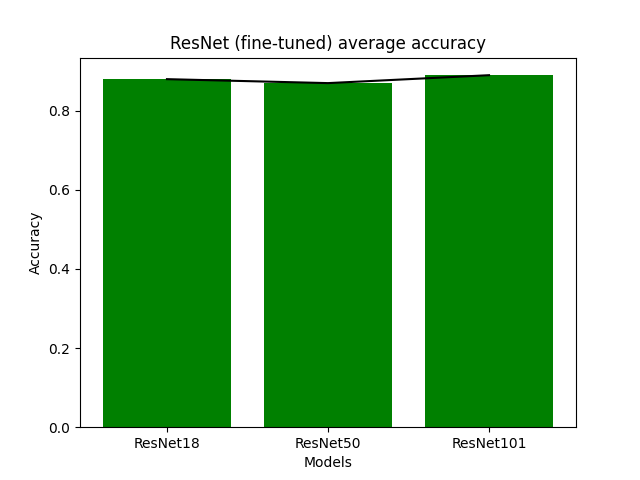
\includegraphics[width=0.6\textwidth]{thesis_assets/plots/resnet_finetuned_average.png}
%     \caption{Average accuracy for fine-tuned ResNet architectures on ant head image dataset.}
%     \label{fig:fresnet_results}
% \end{figure}

\section{The analysis with visualization}

The results in the previous sections show that the fine-tuned ResNet models
outperform the VGG and randomly initialized ResNet models on the task of ant
head image classification. It should be noted that due to the class imbalance in
the dataset, the F1 score is the preferable metric to the accuracy. On average,
the fine-tuned ResNet101 model performed the best with an average F1 score of
0.92. We further analyze the separation learned by both ResNet101 models in the
following section.

\subsection{t-SNE Visualization}

\begin{figure}[h]
    \centering
    \begin{subfigure}{.45\textwidth}
        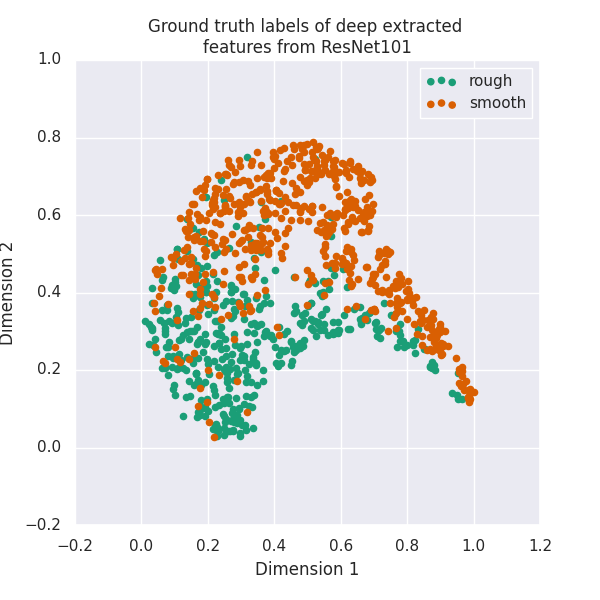
\includegraphics[width=1\linewidth]{thesis_assets/plots/resnet101_gt_tsne.png}
        % \caption{Ground truth labels}
    \end{subfigure}
    \begin{subfigure}{.45\textwidth}
        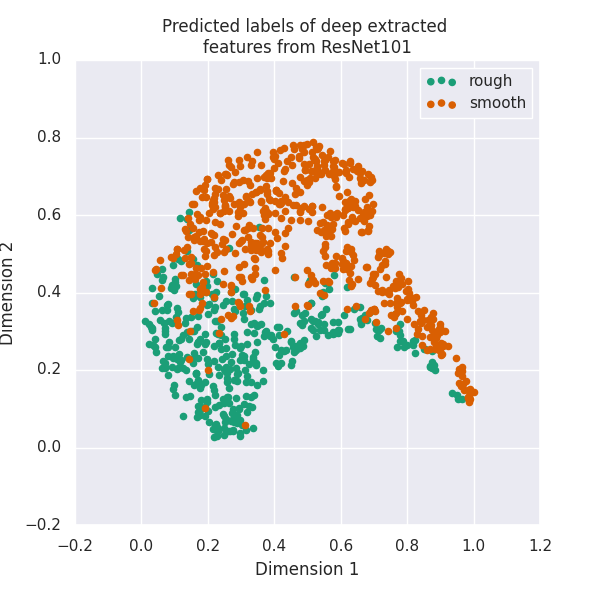
\includegraphics[width=1\linewidth]{thesis_assets/plots/resnet101_pred_tsne.png}
        % \caption{Predicted labels}
    \end{subfigure}
    \caption{t-SNE visualization of the embeddings of the second to last layer
        of the randomly initialized ResNet101 model trained on ant head image
        dataset.}
    \label{fig:resnet101_tsne}
\end{figure}

In this section, we provide visualization of the fine-tuned ResNet101 model and
the randomly initialized ResNet101 model using t-SNE dimensionality reduction.
First, we run the dataset preprocessing method and initialize both models. Then,
both models are trained according to the training parameters and the state of
each model is saved. To visualize the deep extracted features, we modify each
model to obtain the embeddings of the second to last layer. Then, we use the
t-SNE algorithm to reduce the dimensionality of the embeddings to 2 dimensions.
We plot side-by-side the ground truth and predicted labels for each model.
Figure \ref{fig:resnet101_tsne} shows the results of the trained randomly
initialized model and Figure \ref{fig:fresnet101_tsne} shows the results of the
fine-tuned model.

\begin{figure}[h]
    \centering
    \begin{subfigure}{.45\textwidth}
        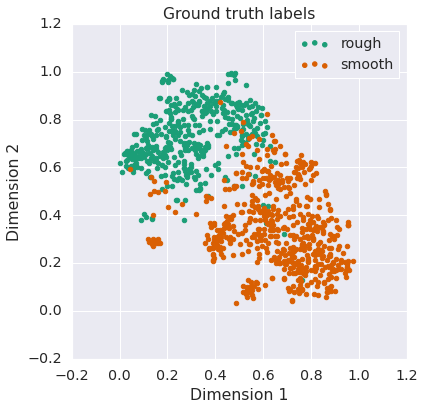
\includegraphics[width=1\linewidth]{thesis_assets/plots/fresnet101_gt_tsne.png}
        % \caption{Ground truth labels}
    \end{subfigure}
    \begin{subfigure}{.45\textwidth}
        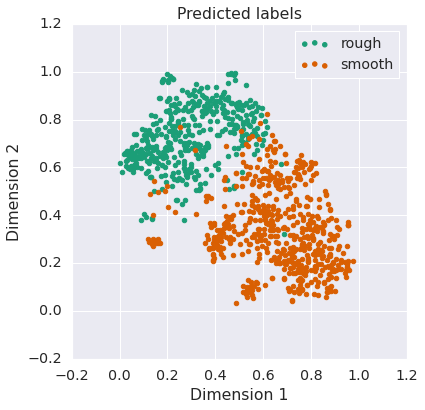
\includegraphics[width=1\linewidth]{thesis_assets/plots/fresnet101_pred_tsne.png}
        % \caption{Predicted labels}
    \end{subfigure}
    \caption{t-SNE visualization of the embeddings of the second to last layer
        of the fine-tuned ResNet101 model trained on ant head image dataset.}
    \label{fig:fresnet101_tsne}
\end{figure}

Based on the visual results of the t-SNE visualization, we can see that the
fine-tuned model learned a stronger separation of the two classes, which
reinforces the results that the fine-tuned model received a higher average
accuracy.

\subsection{GradCAM Visualization}

In this section, we provide some visual analysis of some correctly and
incorrectly classified images using GradCAM. We provide two categories and two
subcategories in our analysis. The two categories are correct and incorrect
classification. Regardless of the feature activation map, the correctly
classified images have the same predicted label as the ground truth, and
incorrectly classified images have different predicted labels. The two
subcategories are ideal and non-ideal feature activation. In the ideal case, the
features that are used to compute the classification are the same as the
features used by the assistants in the sculpture identification process. In
general, the features used by the assistants are the textures of the cuticle on
the ant head. In the non-ideal case, the features used to compute the
classification are not from the head, for example, from the background,
extraneous text, or the body of the ant. We used randomly selected images from
the dataset and the fine-tuned ResNet101 model to perform the analysis. We show
the GradCAM results in Figures \ref{fig:correct_ideal},
\ref{fig:correct_nonideal}, \ref{fig:incorrect_ideal}, and
\ref{fig:incorrect_nonideal}. The left image shows the preprocessed image input
to the model. The right image shows the GradCAM output based on the
classification. Four specimens were selected randomly from each category and
subcategory.

Correctly classified images which use ideal features show the ideal performance
of the model. Incorrectly classified images which use ideal features should be
further analyzed. In essence, the model in this situation knows \textit{where}
to look, but not \textit{what} to look for. In Figure
\ref{fig:incorrect_ideal_84}, the features activated are mostly in the correct
location on the ant head, and the rough texture is clearly visible, yet the
model predicts the incorrect class \textit{smooth}. Similarly in Figure
\ref{fig:incorrect_ideal_177}, the features activated are also mostly in the
correct location, yet the model predicts the incorrect class \textit{smooth}. In
this case, it may be due to the pose of the ant being slightly different from
the average pose. In the incorrectly classified images with non-ideal features,
analysis shows that the model is unable to find \textit{where} to look, and
obtains feature information from other parts of the ant or the background. Cases
where the image was correctly classified using the non-ideal features can
basically be seen as noise. In order to further analyze this class, we should
introduce some parameter such as model confidence to examine further.

\newcommand{\subwidth}{0.35\textwidth}
\begin{figure}
    \centering
    \begin{subfigure}{\subwidth}
        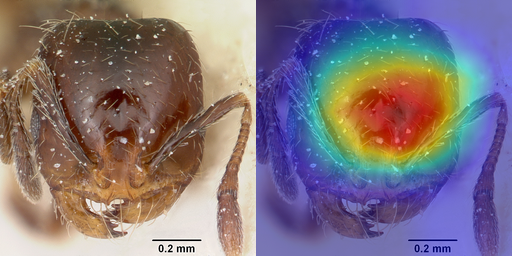
\includegraphics[width=1\linewidth]{thesis_assets/gradcam/correct_ideal/518.png}
        \caption{Ground truth: smooth}
        \label{fig:correct_ideal_518}
    \end{subfigure}
    \begin{subfigure}{\subwidth}
        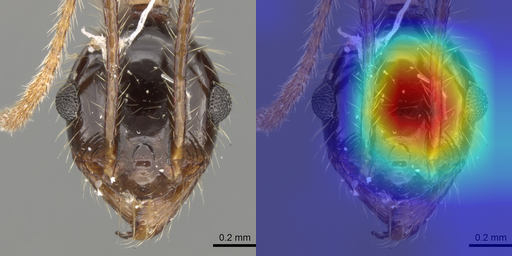
\includegraphics[width=1\linewidth]{thesis_assets/gradcam/correct_ideal/808.png}
        \caption{Ground truth: smooth}
        \label{fig:correct_ideal_808}
    \end{subfigure}
    \begin{subfigure}{\subwidth}
        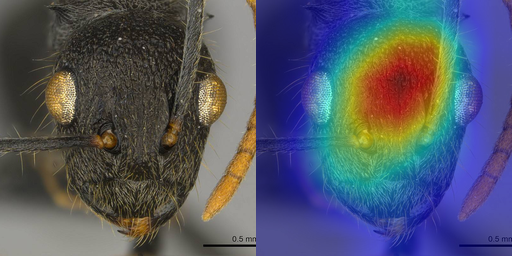
\includegraphics[width=1\linewidth]{thesis_assets/gradcam/correct_ideal/842.png}
        \caption{Ground truth: rough}
        \label{fig:correct_ideal_842}
    \end{subfigure}
    \begin{subfigure}{\subwidth}
        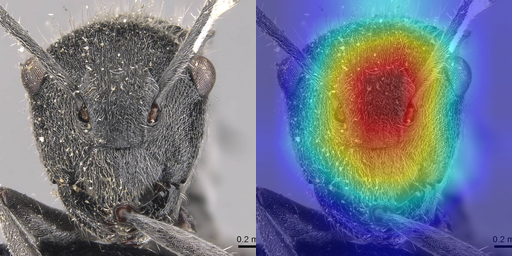
\includegraphics[width=1\linewidth]{thesis_assets/gradcam/correct_ideal/1091.png}
        \caption{Ground truth: rough}
        \label{fig:correct_ideal_1091}
    \end{subfigure}
    \caption{Correctly classified images using ideal features.}
    \label{fig:correct_ideal}
\end{figure}

\begin{figure}
    \centering
    \begin{subfigure}{\subwidth}
        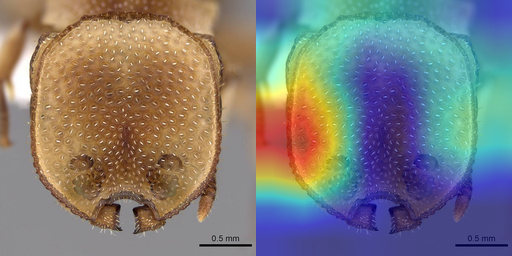
\includegraphics[width=1\linewidth]{thesis_assets/gradcam/correct_nonideal/346.png}
        \caption{Ground truth: rough}
        \label{fig:correct_nonideal_346}
    \end{subfigure}
    \begin{subfigure}{\subwidth}
        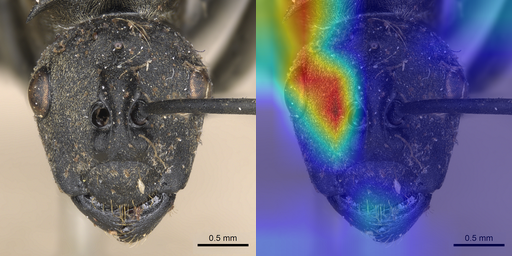
\includegraphics[width=1\linewidth]{thesis_assets/gradcam/correct_nonideal/1554.png}
        \caption{Ground truth: rough}
        \label{fig:correct_nonideal_1554}
    \end{subfigure}
    \begin{subfigure}{\subwidth}
        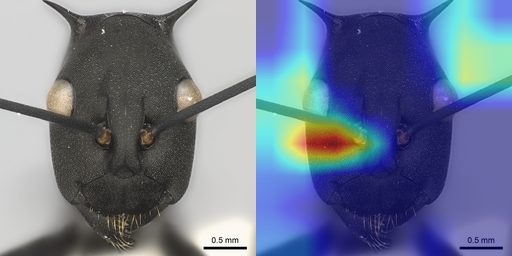
\includegraphics[width=1\linewidth]{thesis_assets/gradcam/correct_nonideal/1694.png}
        \caption{Ground truth: rough}
        \label{fig:correct_nonideal_1694}
    \end{subfigure}
    \begin{subfigure}{\subwidth}
        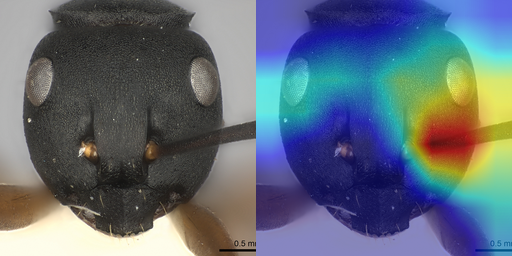
\includegraphics[width=1\linewidth]{thesis_assets/gradcam/correct_nonideal/388.png}
        \caption{Ground truth: smooth}
        \label{fig:correct_nonideal_388}
    \end{subfigure}
    \caption{Correctly classified images using non-ideal features.}
    \label{fig:correct_nonideal}
\end{figure}

\begin{figure}
    \centering
    \begin{subfigure}{\subwidth}
        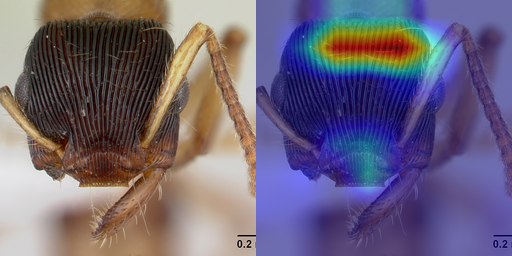
\includegraphics[width=1\linewidth]{thesis_assets/gradcam/incorrect_ideal/84.png}
        \caption{Ground truth: rough}
        \label{fig:incorrect_ideal_84}
    \end{subfigure}
    \begin{subfigure}{\subwidth}
        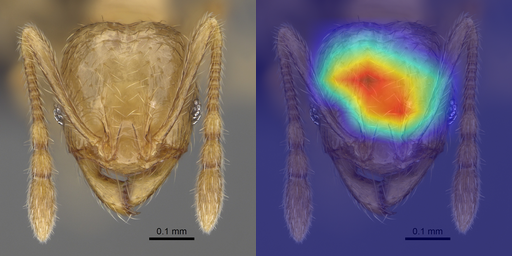
\includegraphics[width=1\linewidth]{thesis_assets/gradcam/incorrect_ideal/86.png}
        \caption{Ground truth: smooth}
        \label{fig:incorrect_ideal_86}
    \end{subfigure}
    \begin{subfigure}{\subwidth}
        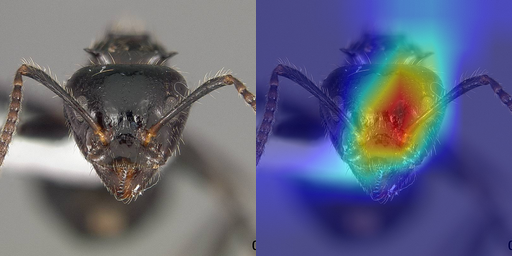
\includegraphics[width=1\linewidth]{thesis_assets/gradcam/incorrect_ideal/177.png}
        \caption{Ground truth: smooth}
        \label{fig:incorrect_ideal_177}
    \end{subfigure}
    \begin{subfigure}{\subwidth}
        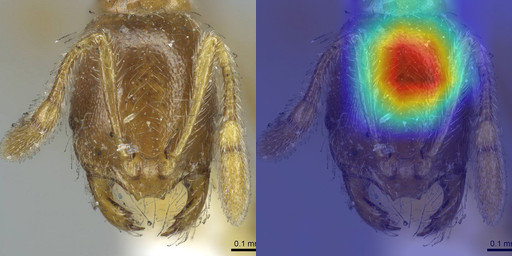
\includegraphics[width=1\linewidth]{thesis_assets/gradcam/incorrect_ideal/197.png}
        \caption{Ground truth: smooth}
        \label{fig:incorrect_ideal_197}
    \end{subfigure}
    \caption{Incorrectly classified images using ideal features.}
    \label{fig:incorrect_ideal}
\end{figure}

\begin{figure}
    \centering
    \begin{subfigure}{\subwidth}
        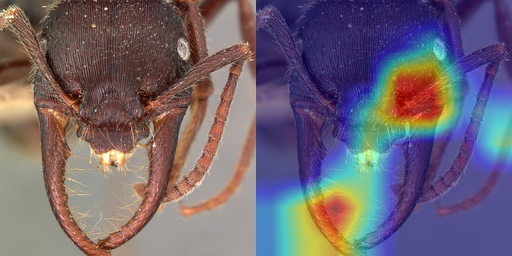
\includegraphics[width=1\linewidth]{thesis_assets/gradcam/incorrect_nonideal/1.png}
        \caption{Ground truth: rough}
        \label{fig:incorrect_nonideal_1}
    \end{subfigure}
    \begin{subfigure}{\subwidth}
        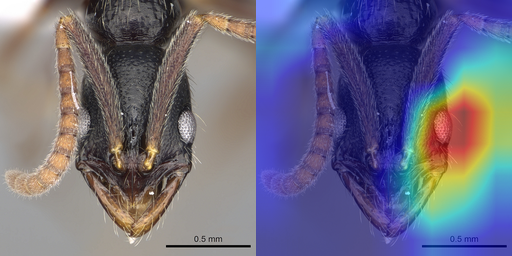
\includegraphics[width=1\linewidth]{thesis_assets/gradcam/incorrect_nonideal/22.png}
        \caption{Ground truth: rough}
        \label{fig:incorrect_nonideal_22}
    \end{subfigure}
    \begin{subfigure}{\subwidth}
        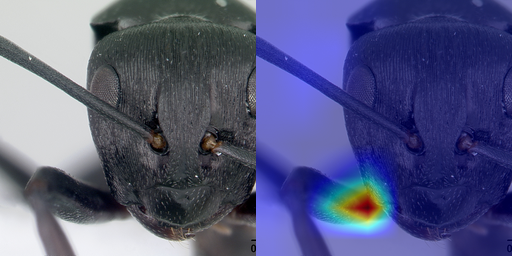
\includegraphics[width=1\linewidth]{thesis_assets/gradcam/incorrect_nonideal/61.png}
        \caption{Ground truth: rough}
        \label{fig:incorrect_nonideal_61}
    \end{subfigure}
    \begin{subfigure}{\subwidth}
        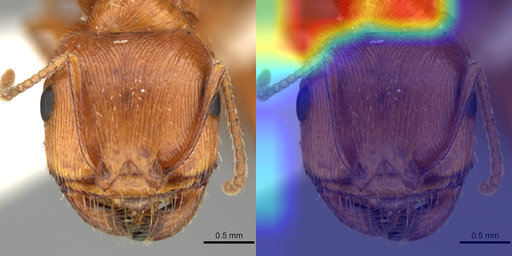
\includegraphics[width=1\linewidth]{thesis_assets/gradcam/incorrect_nonideal/204.png}
        \caption{Ground truth: rough}
        \label{fig:incorrect_nonideal_204}
    \end{subfigure}
    \caption{Incorrectly classified images using non-ideal features.}
    \label{fig:incorrect_nonideal}
\end{figure}

\FloatBarrier
% \clearpage
\section{Conclusion}
Ant cuticle texture presumably has some function, but without the proper tools,
evaluating the function based on thousands of species is infeasible. We have
shown in this work that a deep learning approach and classical image texture
analysis methods can be used to automatically categorize ants based on their
cuticle texture, therefore supporting research on the evaluation of the function
in future work. Our categorization system is novel in the field of automated
insect identification due to the broad number of species captured by it.
Additionally, a model that is pre-trained on a diverse image task such as ResNet
can be transferred to our domain of texture analysis. All code is publicly
available on GitHub (https://github.com/ngngardner/cuticulus).

\bibliographystyle{AIMS}
\bibliography{main.bib,article.bib}
\end{document}
